\chapter{Introduction}

The aggressive development in the industry in the past few centuries brought humankind to an unprecedented advanced stage. We make gas-powered cars allowing us to run faster than any animals on the earth; ships carrying people cruise across the oceans every day, and even spacecraft to escape from Earth and Sun to deep space. But those brilliant achievements came with prices. One of them is the increasing number of wastes in the marine area.

\section{Background} \label{sec:background}

There is a giant plastic waste island called the Great Pacific Garbage Patch on the earth. Its size is 1.6 million $km^2$, more than twice the size of Texas (approximate 0.7 million $km^2$) \cite{Lebreton2018}. This floating waste "continent" is the outcome of the increasing amount of trash produced by industries and individuals in the past centuries and the weak effort of collecting trash in the water.

Compared with the ocean trash problem, coastal pollution is never more severe in history. According to a 2014 research, even in the most remote area on the earth, traces of plastic wastes were found \cite{Cozar10239}. It means while we enjoy using plastic forks and bottles, they have surrounded our planet silently. As factories and manufacturers increase their production, more and more plastic wastes will enter the water in the next few decades. Research shows there will be more plastic than fish in 2050 \cite{agenda2016new}. Figure \ref{fig:01plastic} shows the exact situation that plastic wastes are changing the living environment of sea creatures.

Compared with metal materials, plastic materials are superior in weight and durability and are pretty easy to form in any shape. However, this also makes plastic the most stubborn trash on the earth. Some of them cannot be decomposed in hundreds of years \cite{acssuschemeng.9b06635}. So we must take action on the marine trash collection instead of hoping them go away one day.

\begin{figure}[ht]
    \centering
    \includegraphics[width=.8\textwidth]{01plastic.jpg}
    \caption{Some fishes lives with plastic wastes in water.}
    \label{fig:01plastic}
\end{figure}

\section{Plastic harms}

Most of the marine wastes are made of plastics \cite{Lebreton2018}, as they are resistant to corrosion, oxidation, and corruption. Plastic wastes can kill sea creatures in three main ways:

\begin{itemize}
    \item \textbf{Plastic ingestion}. According to the research, fishes in the North Atlantic area ingest thousands of tons of plastic wastes every year, most of which are microplastics. These plastic grains cause intestine bleeding, which can lead sea animals to death. \cite{Davisonmeps09142}
    \item \textbf{Physical harm}.  Some sea creatures like turtles and birds do not own the ability to remove the plastic bags wrapped around their heads, and they may die of suffocation. Another example of the physical damage of plastics is the derelict nylon fishnet lines. It can entangle even giant animals like seals, whales and leave them stranded.
    \item \textbf{Block the sun light}. Tiny algae in the shallow water layer rely on the sunlight to grow and reproduce. Floating wastes block the sunlight, in turn reducing the number of algae. As a result, there is not enough food for small sea animals, the bottom residents of the food chain. The reduction in food limits the overall animal population. On the other hand, fewer plants mean less oxygen. The dissolved oxygen in water also drops, making fishes harder to breathe.
\end{itemize}

\section{Plastics on the shorelines}

There is research pointing out the vast majority of the plastics in the ocean end up washed, or buried under the shorelines, whether dry shorelines, coastal areas, or offshore areas \cite{owidplasticpollution}. However, because shorelines are long and most parts are far from human habitats, the trash collection force on shorelines is significantly less than the land. The main reason is the lack of hands and the high price of human labor.

That is why we designed Piranha. Piranha is a water surface robot that can be operated remotely by a human worker or cruise on its own to collect floating trash near the coast. It has a highly advanced control system built similarly to modern drone controllers, and we equipped it with customized control algorithms. On the mechanical side, it has a straightforward design to achieve lower building costs and higher reliability. 

Figure \ref{fig:01rendered} shows a rendered model of Piranha made in SOLIDWORKS 2017. Figure \ref{fig:01piranha} shows the overall structure of Piranha during the fourth field test. In that test, we tried using a pulley system to lift the collection bin so that human workers could easily dump the trash when the trash bin was full.

\begin{figure}[H]
    \centering
    \includegraphics[width=.6\textwidth]{01rendered.png}
    \caption{Piranha rendered model, only the floats and frames are shown.}
    \label{fig:01rendered}
\end{figure}

\begin{figure}[H]
    \centering
    \includegraphics[width=.6\textwidth]{01piranha.jpg}
    \caption{Piranha during the forth pond test in July, 2021.}
    \label{fig:01piranha}
\end{figure}

\section{Trash collection systems}

Trash collection is the core function of Piranha. While Piranha used the simplest way to collect trash, we had several other options in the early development stage. In this section, I will introduce these different kinds of trash collection systems in the hope of inspiring more ideas from the readers.

\subsection{Venturi Pump}

The device shown in Figure \ref{fig:01air_pump} is a simplified model of a Venturi pump trash collection system. The compressed air has a leftward momentum, pushing the water to flow. As a result, the trash is captured by the water current and trapped by the net near the tube.

The advantage of this design is that there is no physical contact between the moving parts and the trash, so the chance of being stuck by the debris is relatively low. And compressed air, on the other hand, gives the boat driving power, so the thrusters are not needed anymore. These advantages are essential because driving among floating trashes with thrusters is dangerous. Ropes, plastic bags can easily get caught by the thrusters and stop the motor, which in the end leads to a complete power system failure.

However, the disadvantages of this system are that the complexity of the system and the low efficiency.  The air pump needs too much power compared with the underwater propellers. A common airboat has a 3-5 MPG fuel efficiency rating. Given by today's battery technology, it is unrealistic to drive the airboat with electricity instead of gasoline.

\begin{figure}[H]
    \centering
    \includegraphics[width=.5\textwidth]{images/01air_pump.pdf}
    \caption{A simplified model of Venturi pump collection system. We fixed the capture net near the dotted lines. Pink stars represent the floating trashes in water. The pressure drop along the channel forces water to flow because of the Venturi effect.}
    \label{fig:01air_pump}
\end{figure}

\subsection{Conveyor}

The conveyor is the most common solution in collecting floating trashes and algae. Because if we separate the collection part from the trash container, then the trash volume depends on the container only. And the mechanical design is more straightforward compared with the Venturi pump solution. A simple combination of a passive roller and a motorized roller is enough. The conveyor-based trash collection system is shown in Figure \ref{fig:01conveyor}.

\begin{figure}[H]
    \centering
    \resizebox{.5\textwidth}{!}{\input{images/01conveyor.pdf_tex}}
    \caption{A Conveyor collection system illustration. The upper roller is motorized; meanwhile, the lower roller is passive. Pink stars and the green bucket represent the trashes to be collected and the trash container, respectively.}
    \label{fig:01conveyor}
\end{figure}

\begin{figure}[H]
    \centering
    \includegraphics[width=.8\textwidth]{01orca_in_water.jpg}
    \caption{A concept model of Piranha using the conveyor collection system.}
    \label{fig:01orca_in_water}
\end{figure}

However, this configuration is usually seen on large-sized boats because there are too many moving parts, and the cost is considerably higher than other options. On Piranha, we did try the conveyor configuration as the model shown in the Figure \ref{fig:01orca_in_water}. However, due to the high cost and the difficulty in manufacturing, we decided not to adopt this design at the early development stage.

\subsection{Mesh bucket}

The collection bucket is made of meshes and allows water to go through but not trashes. This collection system is passive, meaning the boat needs to carry the bucket and drive around to collect trashes.

This solution is the simplest of all choices, and the cost is low. However, it does have several drawbacks. One of them is the capacity of the mesh bucket limits the total trash carried by Piranha in one run. Second, the bucket is submerged in water, making it very hard for workers to empty the bucket at the dumpsite. Last by most important, because the bucket does not provide any active forces on the already captured trash, there is no guarantee that the garbage will not come out of the bucket if the boat drives backward.

Piranha has a simple lever system to avoid the last two issues. The lever system illustration is shown in Figure \ref{fig:01lever-net}.

\begin{figure}[H]
    \centering
    \includegraphics[width=.8\textwidth]{images/01lever-net.png}
    \caption{On the left part, the Piranha is driving forward. On the right part, Piranha is moving backward.}
    \label{fig:01lever-net}
\end{figure}

We carefully designed the lever so that it is nearly perfectly balanced in the vertical position. A minor disturbance will change the angle of the pole. As shown in the left part of the figure, if Piranha drives forward, the rod is vertical because of the water pressure on the lower part. The net's mouth opens in the vertical direction, and trash starts to flow inside the bag.

The right part shows the situation when Piranha drives backward. The lower part starts moving up due to the water pressure. The mouth of the net leaves the water so that the trash cannot escape. In such a way, the lever automatically "seals" the net when the Piranha starts driving backward or the water current is faster than the boat and is about to bring out the trash. 

\section{Similar Robots}

Some other robots can do a similar job as Piranha at the time when we designed Piranha. Almost all of them have one of the configurations mentioned in the previous section. However, they vary in some subtle details when it comes to the goals and technologies behind them.

\subsection{WasteShark}

Sponsored by the Robotics Innovation Center in Germany and the European Union, WasteShark has a very similar design to Piranha. They claimed WasteShark could carry 350-kilogram trash in one run. It also has a special navigation algorithm to allow the robot to return to the dock once the bucket is full. Several water quality sensors on the boat can detect the water quality data, including pH, ORP, conductivity, dissolved oxygen, turbidity, ammonium, chloride, nitrate, salinity, mV, ORP, TDS, resistivity level, and send them back to the data center\cite{SCHMALTZ2020106067}.

\subsection{Clearbot}

Clearbot shown in Figure \ref{fig:01clearbot} is an intelligent robot designed by a company in Hong Kong. It is very similar to Piranha, except it used a conveyor instead of a mesh bucket. According to the description provided on their website, Clearbot has a self-driving function and a computer and camera to identify the type of garbage and upload the data to a cloud-based platform.

Clearbot's primary function is collecting trash from the water, cleaning the rivers and oceans globally. Besides that, it can also identify a wide range of waste and material types to help the recycling companies to classify the trashes. According to the recent updates, the developers of Clearbot are working on the swarm algorithm for the robot.

\begin{figure}[H]
    \centering
    \includegraphics[width=.6\textwidth]{01clearbot.png}
    \caption{Clearbot.}
    \label{fig:01clearbot}
\end{figure}